% Chapter 1

\chapter{Introduction} % Write in your own chapter title
\label{Chapter:Intro}
\lhead{Chapter 1. \emph{Introduction}} % Write in your own chapter title to set the page header

\section{Motivation}
\label{sec:Motivation}

\subsection{The answer we seek.}
%Why did people first start looking at galaxies
The firmament has been the muse of humans for as long as we have recorded our history and most likely longer still. The field of astronomy is descended from priests who worshiped celestial objects as the divine and sought for them to bring meaning to their world. Structures such as Stonehenge use celestial objects to allow people to track the `repetitious' passage of time, thus being able to predict the seasons. It is possible that this correlation between the heavens and the earthly systems so critical to life, is the reason that humanity became convinced that universe was there for our benefit. Elaborate orrerys with the earth at the center of all creation were built to explain how the sun and planets orbit around us cementing our belief that we are at its origin. The progression to modern astronomy was slow, however, now instead of assuming the universe was built for humans we now try to discover our place amongst a cosmos that is unfathomably enormous, diverse and inhospitable. 

The Milky Way is our home and was the first observed galaxy. The name comes from Greek to mean `milky circle' stemming from our belief that the universe exists to give us life and gives the galaxy a mammalian nurturing characteristic. The idea of complexity emerging from the universe is present in the first classification of the structures of galaxies by Edwin Hubble \citep{Hubble1926Extra-galacticNebulae.,Hubble1927TheNebulae}. Complex spirals were thought to be the descendants of elliptical galaxies leading to the misnomer of 'early type' (elliptical) and 'late type' (spiral) galaxies, as it has since been found that it is in fact spiral galaxies that transform into elliptical galaxies. The Universe is at it's core in antithesis to the way humanity regards themselves, it thus presents a challenge in thinking to detach hubris and think logically about a system that in its entirety is truly incomprehensible. We must always strive to detach our personal identity from our analysis of the cosmos or be forever constrained by the bias inherent to the human condition.

Most advances in astronomy have come from technological progress. When the most advanced way to view the cosmos was by simply looking upward we knew little of what there was and interpreted as best we could. With the advent of optics, such as lenses and then mirrors, leading to the building of telescopes the ability to look deeper into the heavens become a possibility and the first work on classification was done. Modern advances such as CCD/SED photographic plates, and telescopes that work outside of the visible light spectrum information, give information far beyond what the human eye can see. The more information we gather the more theories of formation come to be, the emergent complexity of Hubble gives way to hierarchical formation destroying structure, galaxies are found to be the birthplace of stars like our sun and where some galaxies are forming many stars some appear dead, looking backwards in time astronomers find the cosmos appears to have passed the peak of creation with galaxies on average forming less stars now then ever before. The one thing that connects all astronomers over all ages is the desire to answer the ultimate question of `why?'.

%How has the study of galaxies progressed
\subsection{The tools we use.}
The field of astronomy is somewhat unique in science in that all our data and `experiments' already exist are sought out through observation. Often the hypothesis follows the data in contrary to the scientific method of collecting data to support a hypothesis. Furthermore, for galactic astronomers objects observed are effectively frozen in time, the timescales galaxies evolve on eclipse not only a human lifespan but the entirety of human civilization. It is our good fortune that the `cosmic speed limit', the speed of light, means the further away from earth we look the further back in time and into the history of galaxy formation. By looking at galaxies at many different epochs we are able to construct a picture of how the galactic population has changed and evolved. Theories of how the early universe transforms in to the universe we see locally emerged and a tools were required to test these theories that could show galactic formation on human timescales. The first such model by \citet{Holmberg1941OnProcedure.} predates digital computing using an array of light bulbs using the `candle power' to proxy mass and evolving the system using gravitational arguments and confirms the hypothesis that in distributed merging systems the loss of energy during a encounter results in a capture or merger as we know it today.

With the rapid increase in computing power over the last century, the capability of the simulation of galaxies has grown. More than simply testing the dynamics of mass, simulations now have prescriptions for the formation of gas from stars, the mergers of complex systems of tens of galaxies in a full cosmological setting, the feedback of energy from central black holes millions of times the mass of our sun, and more... \citep[e.g.,][]{McAlpine2015TheCatalogues, Pillepich2018FirstGalaxies}. However advanced these models have become a full understanding of our Universe still seems to be beyond our capability. Other less computationally intensive tools have been used to try to understand from first principles the formation of our Universe, using mathematical analytics to model galaxy formation. Since their original inception where galaxies form from gas via the loss of angular momentum and cooling to form galactic disks \cite{Mo1998TheDiscs}, these so called Semi-Analytic Models have branched out to cover tens of different analytics that try to balance different processes to faithfully recreate as many observable galaxy properties as possible \citep[e.g.,][]{DeLucia2006TheGalaxies, Guo2011FromCosmology}. The most recent development in galactic modelling is more humble in it's approach, seeing not to recreate the entire universe but to use what we observe as a guide. These Semi-Empirical Models constrain the model as much as possible using observations and then ask focused questions to understand if our hypothesis of formation adequately link the observed galactic population over cosmic history \citep{Hopkins2010MERGERSMATTER, Zavala2012, Moster2013, Shankar2014, Moster2018Emerge10}.

%What questions will we answer
\subsection{The questions we answer.}
In this thesis we describe $\steel$, the STastical sEmi-Empirical modeL, PJG's contribution to the galactic modelling community. \steel has been designed to be in complement to the existing models of galaxy formation evolution and environment. \steel is based on semi-empirical modeling techniques but its defining characteristic is its statistical nature. Traditional models, described in more detail below, simulate: a cosmological volume, a catalogue of objects extracted from a cosmological volume, or a catalogue of objects generated to mimic a cosmological volume. \steel goes against this trend creating a simulation of the universe using number density functions to describe cosmological volumes without the volume and resolution constraint that effects discrete object simulations. The full methodology for \steel is given in Chapter \ref{Chapter:STEEL}. The advantage of having a volume free model is twofold, firstly, we can simulate rare objects that have a number density far lower than can be captured in traditional models, secondly, in a traditional model objects that appear with a high number density are simulated orders of magnitude more often than objects with low number density not only is this computationally inefficient it is a source of bias. 

\section{$\Lambda$CDM Cosmology}
\label{sec:LCDM}
%Why do we think dark matter exists
Dark Matter is a theorized form of matter that interacts only though gravity and is therefore not observable with traditional methods that rely on photons. The first notion of dark matter was from \citet{Zwicky1933DieNebeln}, it was observed that the binding mass required to hold the Coma Cluster together was roughly 400 times the observable stellar mass. It took many years and observations of the motions of satellites around our own galaxy also requiring an extended unseen matter structure until the ideas of dark matter begun to take hold. Further evidence was mounted by observing the rotation curves of galaxies \citep{Roberts1973ComparisonTypes}, the rotation of the outer regions of the galaxy did not fall off as the mass profile of the luminous galaxy should suggest. Whilst there exist other theories such as Modified Newtonian Dynamics (MOND), that suggests gravity acts differently at large scales, dark matter is now the preferred model amoungst physicists to explain the mass deficit in the Universe. 

%What is LCDM
Once one accepts a type of matter that exits everywhere, is 5 times more abundant than baryonic matter, and does not appear to give out any electromagnetic signature the first logical question becomes ``What is it?''. To this day we do not know the precise nature of dark matter only some constraints to say what it is not. Initial thoughts suggested brown dwarf stars or black holes, dark yet familiar objects that satisfy both adding mass and not being visible. It is now thought that dark matter consists of a massive subatomic particle due to the proposed sizes of these particles they must inherently have a lower thermal velocity hence they became known as cold dark matter (CDM). By combining the formation model with the cosmological constant ($\Lambda$) to create a flat universe, \LCDM is born. 

%What are the predictions of LCDM
The prediction from \LCDM of foremost importance to galactic modelling is that of hierarchical assembly. Dark matter collapses under gravity from an initial density field, that mimics the cosmic microwave background. This means that areas of greater density collapse faster and eventually attract other collapsed regions further increasing their mass. This structure has become commonly referred to as the `cosmic web'. As dark matter interacts only via gravity it is relatively easy to simulate on large scales, as such there have been many massive simulations of \LCDM volumes in various cosmologies (WMAP5, Planck), of note are the Millennium simulation \citep{Boylan-Kolchin2009ResolvingSimulation} and the Bolshoi/MultiDark simulations \citep{Klypin2016}. We show a visulisation of the Bolshoi Plank dark matter simulation in \ref{fig:DMStruct}, the `cosmic web' is made visible dark matter halos seen here as the darkest regions are connected by filamentary structure. There is a notable void in the upper right of the image and two clusters one in the top middle and one in the bottom left. The initial dark matter distribution is accentuated by giga-years of collapse creating the complex structure seen.

\begin{figure}[h]
	\centering
	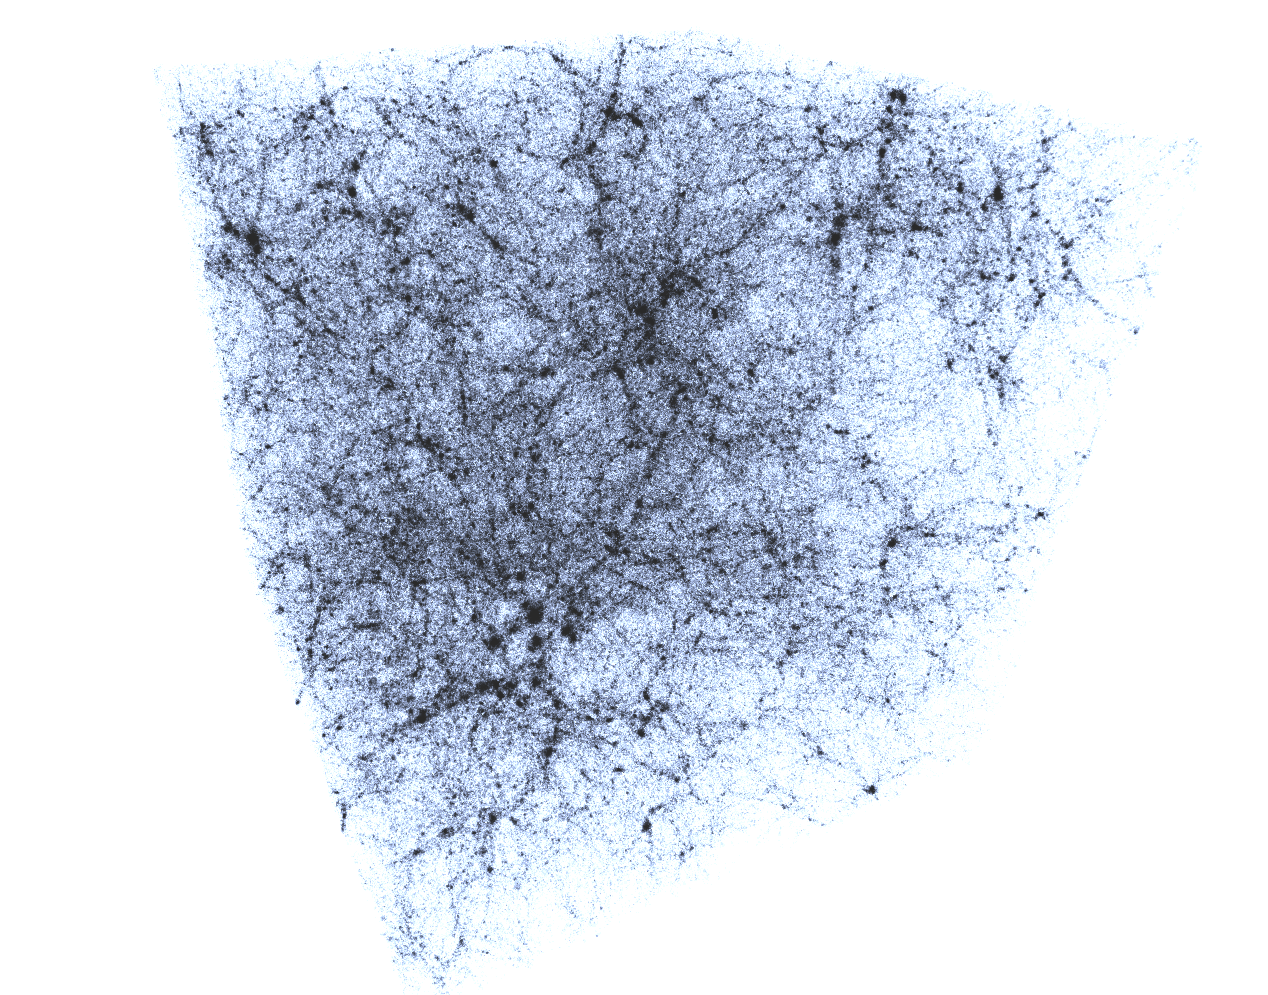
\includegraphics[width = \linewidth]{Figures/Chapter1/DMStruct.png}
    \caption{A visualization of the `cosmic web'. The shading shows the distribution of dark matter. The darkest regions are the spherical `halos' between the halos extended filaments can be seen. Regions of note are the void in the upper right and the clusters in the top middle and lower left, initially the dark matter density field would have been simmilar to the microwave background but giga-years of collapse have accentuated small features into large structure. Image Credit: C.Marsden using the galaxy and structure visualization code Astera processing the Bolshoi Planck dark matter simulation (https://astera.soton.ac.uk/).}
	\label{fig:DMStruct}
\end{figure}

%Halo Finders, Halo mass functions, Merger Trees and EPS formalism
To be able to analyze the complex dark matter structure objects must be classified, the dark matter haloes, from simulations, that form the basis of many galaxy formation models can be classified in two ways. Firstly, virialized haloes collections of dark matter particles\footnote{Note here a dark matter particle is a simulation element, often millions of solar masses, and not the theorized fundamental particle.} that are balanced in terms of their potential and kinetic energy, mathematically, 
\begin{equation}
    \langle T \rangle = -\frac{1}{2}\sum^{N}_{k=1}\langle \bold{F}_k \cdot \bold{r}_k \rangle.
\end{equation}
Secondly, haloes can be defined by their over density, simply with respect to either the background\footnote{The average density of the Universe.} or critical\footnote{The density required such that the universe will not expand forever.} density a spherical region is picked such that the average mass within this sphere is a set number times that density. For example $M_{200c}$ would be the mass of a halo where the halo is defined as the spherical region that is 200 times the critical density. It is then critical to gain an understanding of how these structures relate to one another. We have already introduced the concept of one halo growing though accretion of another, this is not an instantaneous process during accretion and subsequent cannibalization the smaller halo can be refereed to as a sub-halo. This creates collections of haloes in one space that are commonly referred to as groups or clusters depending on their mass or number of members. It is essential that these structures can be resolved from simulation and thus there have been several methods developed to analyze the simulated dark matter volumes to create catalogues of haloes. 

\begin{itemize}
    \item Bound Density Maximum: BDM classify halo structure by defining a spherical over density threshold e.g. $M_{200c}$ then removes particles that exceed the escape velocity \citep{Klypin1997Particle-MeshSimulations}.
    \item Friends of Friends: FOF uses a halo linking threshold, particles are `linked' together if they are closer than the threshold. One particle cannot be in two FOF groups simultaneously such that groups are unique, by assigning different linking lengths substructures can be identified and a picture of the halo hierarchy built \citep{Davis1985THEMATTER}.
    \item ROCKSTAR (Robust Overdensity Calculation using K-Space Topologically Adaptive Refinement): ROCKSTAR is a cutting edge development of the FOF halo finders, using a 6-dimensional phase space and a temporal dimension the structure and evolution of haloes is extracted from dark matter simulations \citep{Behroozi2013TheCores}.
\end{itemize}

Once identified halos are then classified as central haloes or subhaloes, subhaloes then may contain further structure thus there are different `orders' of halos: $0^{th}$ order or central halos, $1^{st}$ order or sub-halos whose parent is a $0^{th}$ order halo, $2^{nd}$ order or sub-halos whose parent is a $1^{st}$ order halo, and so on. A useful description of the halo distributions are the halo and subhalo mass functions. The halo mass function is usually defined as the number density of central halos at a given mass in a given volume. The subhalo mass function has multiple definitions depending on the application, firstly, one can define the global subhalo mass function simmilar to the halo mass function this is the number density of subhaloes at a given mass in a given volume. Secondly, one can define the subhalo mass function relative to a particular host halo to give the number of subhaloes of a given mass ratio $M_{subhalo}/M_{central}$ one expects to be associated to a halo mass $M_{central}$. As the subhaloes are an evolving population it is important to define which subhalo mass one is using:

\begin{itemize}
    \item Unevolved Subhalo Mass Function (USHMF): This mass function is the total number of subhaloes as a function mass that accreted onto a central halo over its entire history. The subhalo mass is added at the point of accretion and is never evolved and no number density is ever lost. This mass function is useful for understanding the total accretion history of a halo.
    \item Unevolved Surviving Subhalo Mass Function (USHMF): This mass function is the total number of subhaloes as a function mass that exist in a halo at a given epoch. Subhaloes once accreted are not updated in mass but do eventually merge and are then considered removed. This mass function is useful as it retains information about the infall mass and can be further broken down such that one knows the contribution of infall epochs to the total.
    \item Evolved Subahlo Mass function (ESHMF): This mass function is the total number of subhaloes that exist in a halo at a given epoch where the subhaloes have undergone mass loss/transfer to the central halo. This mass function is the `true' subhalo mass function that one would expect to see if dark matter were directly observable.
\end{itemize}

In Figure \ref{fig:SubHaloes_byz}, in the left hand panel we show the halo mass function at redshift $z=0.1$ note the characteristic shecter function shape with a linear relationship between number density and mass in log-log space that breaks and rapidly declines above a threshold mass, here $M_h\sim 10^{14}$ $M_{\odot}$. In the right hand panel we show the Global Unevolved Surviving Subhalo Mass Function at redshift $z=0.1$. In this figure the shading represents the redshift of infall, note the logarithmic scaling means the shading is not linear. Recent accretion is the dominant contributor of subhaloes at all masses, furthermore, for high mass subhaloes $M_h \geq 10^{13} M_{\odot}$ there is no contribution from high redshift accretion.

\begin{figure}[h]
	\centering
	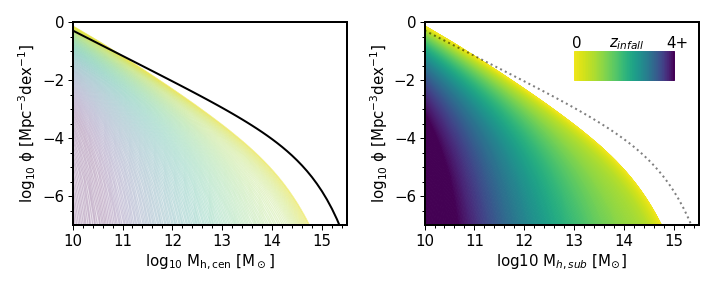
\includegraphics[width = \linewidth]{Figures/Chapter1/SubHaloes_byz.png}
    \caption{Left: We show the Halo Mass function, the global number density of haloes at redshift $z=0.1$. Right: We show the Global Unevolved Surviving Subhalo Mass Function at redshift $z=0.1$. The colour gradient shows the fraction of subhaloes at each mass contributed by redshift of infall, note due to the logarithmic scaling the thinner yellow bar at the top of the distribution is a majority contribution of subhaloes. There is a clear colour gradient from left to right showing that high mass haloes are exclusively contributed by recent accretion. In each panel we show the other mass function for comparison of number density.}
	\label{fig:SubHaloes_byz}
\end{figure}

In addition to the distinction between central and satellite haloes and their number densities, information about the assembly is also gained from simulations. Halo assembly histories are commonly visualized as simple(\textit{ish}) tree network, referred to as a merger tree. Central haloes are identified at a low redshift and the main progenitors followed backwards in time to create the central `trunk', at any epoch where a merger occurs the main progenitor is assigned to be the larger of the two haloes\footnote{This remains true even if the main progenitor branch becomes smaller than the other branch at an earlier redshift.}. At each merger a `branch' is created following this branch gives the history of that subhalo. In this way all the contributing haloes can be visualized. In Figure \ref{fig:SimpleTree} we give a example of a simple merger tree. There are increasingly more complex merger tree diagrams, it is not the case that a haloes merge simply we list some examples and show what these may look like on a stylized merger tree in Figure \ref{fig:Substructures}.

\begin{figure}[h]
	\centering
	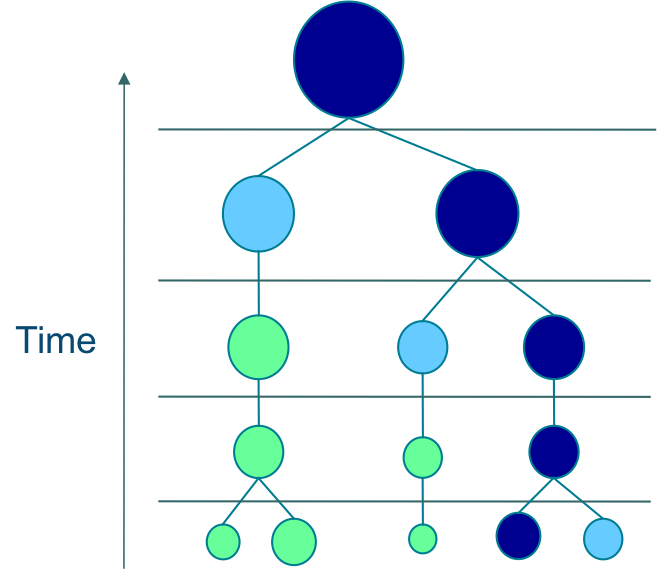
\includegraphics[width = \linewidth]{Figures/Chapter1/Merger_Tree_Simple.png}
    \caption{A cartoon of a simple merger tree. Increasing time moves up the page as indicated on the right, horizontal lines separate epochs. Dark blue circles represent the main progenitor or trunk haloes of the merger tree. Haloes that merge directly onto the trunk are coloured in light blue, the merger history or branch for each of these merging haloes is shown in green.}
	\label{fig:SimpleTree}
\end{figure}

\begin{itemize}
    \item Substructure: A halo is not immediately dissolved upon accretion to the central halo, substructure is therefore maintained in central haloes between epochs. Furthermore, haloes on accretion may also carry substructure this creates 2nd (and above) order substructure.
    \item Flyby Haloes: Some haloes may pass through another halo and loose mass but not be fully captured. These haloes are known as flyby halos and must be accounted for to not over count accretion.
    \item Re-Accreted Haloes: Halos on particularly eccentric orbits or halos with initially high velocity may enter a halo and leave with a large velocity. These halos can then go to a distance where a simulation does not regard them as part of the halo group appearing to be flyby haloes. However, at some later time these halos may reenter the group. One must ensure these halos are not double counted, and that the mass they are accreted at is fit for purpose (i.e., mass at last accretion, mass at first accretion, or peak mass).
\end{itemize}

\begin{figure}[h]
	\centering
	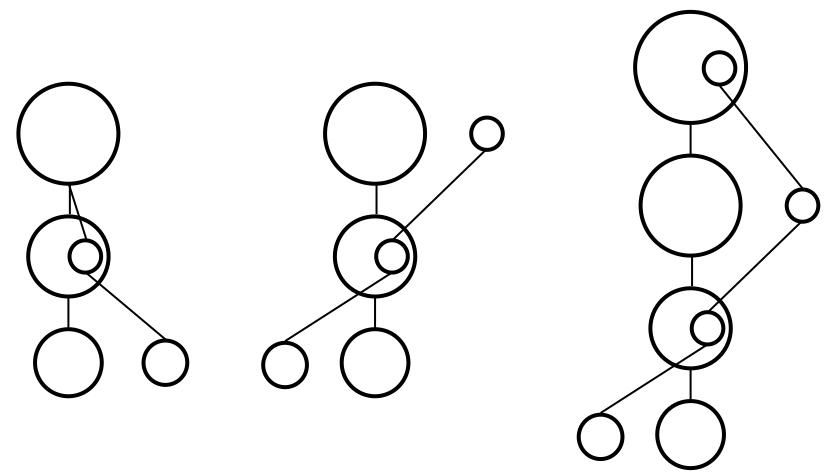
\includegraphics[width = \linewidth]{Figures/Chapter1/Substructures.png}
    \caption{From left to right: An example of, $1^{st}$ order substructure, a Flyby halo, a re-accreted halo.}
	\label{fig:Substructures}
\end{figure}

Whilst there is clearly a wealth of information in large dark matter simulations for many galaxy models that only require the simple dark matter distributions. Press-Schechter Formalism \citep{Press1974} provides an alternative way to generate simple analytic dark matter distributions at a greatly reduced computational cost. For a simple visualization one can consider the dark matter distribution at high redshift as a random Gaussian probability distribution, peaks in this distribution represent dark matter over densities and higher peaks collapse earlier. This can be visualized as a time evolving threshold above which the dark matter is a collapsed halo, if the summation of two gaussians are above this threshold then they are together are collapsed structure created by the merging of two haloes. A simple cartoon is shown to visualize this in Figure \ref{fig:PS_Cartoon}.

\begin{figure}[h]
	\centering
	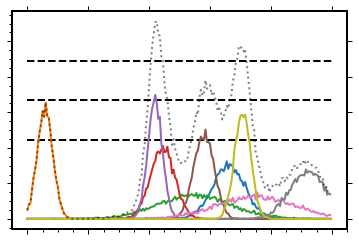
\includegraphics[width = \linewidth]{Figures/Chapter1/PS_Cartoon.png}
    \caption{A visualization of the core theory of Press-Schechter Formalism. The solid coloured lines are random gaussian distributions representing fluctuations in the initial mass density field, the grey dotted line is the total mass distribution, the three black dashed lines are for visualizing the threshold of collapse at different epochs.}
	\label{fig:PS_Cartoon}
\end{figure}

Following Figure \ref{fig:PS_Cartoon} considering the topped dashed line, as the first epoch we look for collapsed haloes, there are two peaks in the density field above the threshold the area above the threshold is related to the size of the halo and the spread the concentration. At the second threshold there is another collapsed peak mostly contributed by the brown gaussian that is close to a peak seen at the previous threshold from the yellow gaussian, furthermore, the two peaks from the first collapse have grown in mass as can be seen by an increased area. Finally, looking at the last collapse threshold,  on the left there is a new isolated peak more importantly on the right the peaks created by the yellow and brown gaussians now create one continuous area above the threshold this is an indication of two merged haloes, there are still two peaks that can be thought of in a simmilar manner to substructure. It is simple to see that at later epochs the merged substructures will also include the purple peak. This picture is a oversimplification of Press-Schechter Formalism, the gaussian field is actually significantly more interesting modeled from the CMB, instead of simple collapse thresholds a window function is used to smooth the density field. 

The Press-Schechter Formalism can be used to analytically build a merger tree by understanding the probability of any two over densities merging one can construct an algorithm that starting at a given redshift with a given mass halo and construct a theoretically valid merger history. we summarize here the \textsc{galform} \citep{Cole2000} method for making merger trees from Press-Schechter Formalism\footnote{In \citet{Parkinson2008GeneratingTrees} improvements to this method are proposed to better align the generated merger trees with the millennium simulation by using a perturbing function to remove systematic differences between N-Body simulations and the algorithm.}.

\begin{itemize}
    \item Pick a starting Mass, $M_{h}$ and redshift $z$. This will be the final mass/redshift for the main progenitor halo in the tree.
    \item Step backwards in redshift in steps, $dz$, where $dz$ is chosen that the probability, $P$, of a halo having a merger in $dz$ is $P\ll1$.
    \item Generate a uniform random number, $N$, if $N<P$ the halo splits, else the mass is reduced to account for unresolved haloes or smooth accretion and the process repeats.
    \item If the halo has split a random number is generated from the probability distribution that defines the possible progenitor halo masses from  Press-Schechter Formalism this is the mass of the split halo, $M_{split}$. The central halo mass is then updated to be less the split mass and a smooth/unresolved accretion component and the process repeated.
\end{itemize}

The merger trees generated using this algorithm are simpler and less computationally expensive and if calibrated properly fully consistent with \LCDM cosmology. They therefore are an ideal choice for simulations that need to generate halo merger trees on demand.

%How do these predictions effect galaxy assembly
Dark matter interacts with baryonic matter via gravity, as dark matter is 5 times more abundant than normal matter it is the dominant gravitational force in the universe, consequently a prediction of \LCDM cosmology is that the baryonic matter traces the dark matter distribution. Galaxies are thought to assemble in the center of dark matter halos where gas accumulates, the larger the halo the larger quantity of gas collects in the halo and the larger the galaxy. The hierarchical assembly of dark matter halos is then translated into the galaxy population, massive galaxies are expected to be surrounded by many smaller satellite galaxies that loose angular momentum to the halo and eventually merge with the central galaxy.

\section{Hydrodynamic and N-Body Simulations}
\label{sec:Hydro}
%What is Hydrodynamics or N body
Hydrodynamical simulations are the most `real' galaxy simulation, dark matter, gas, and stars are assigned to a volume of particles and/or grid cells, forces are then applies to each element with respect to each other element. The volume is then solved by repeated solving and time stepping and snapshots produced at set intervals to be used for analysis. Processes that take place below the resolution limit of the simulation, such as starformation, are simulated using a sub-grid routine based on the properties of the given volume element.

%State of the Art
\subsection{State of the art: Illustris TNG}
The Illustris TNG simulations are a suite of 18 simulations, they use three different volumes, $\sim 50, 100, 300$ ${Mpc}^{3}$, and study a range of physical complexity and resolutions. TNG at its core use the code \textsc{arepo} \citep{Springel2010EMesh} which solves coupled ideal magneto-hydrodynamics and self gravity using periodic boundary conditions. Even for TNG50 where exceptionally high resolution for a cosmological simulation can be achieved much of the baryonic physics falls below the resolution limit, this physics in then included via so called `sub-grid' models. Sub-Grid models are used for star formation, super massive black holes, galaxy feedback process (starformation and AGN) and more. A specific example of one such sub-grid model is star formation, gas above a threshold density $n_H \simeq 0.1cm^{-3}$ is allowed to form stars following the results of \citet{Springel2003CosmologicalFormation}. Sub-grid models attempted to replicate results from smaller higher resolution simulations or from observations. 

%Drawbacks
\subsection{Pros and Cons}
The drawbacks of using a hydrodynamic model are foremost a limitation of resource they require vast amounts of computational resource to run and take a lot of developer time to create. Furthermore, they create huge amounts of output data that can be difficult to process and interpret. The combination of these effects result in a simulation that has volume and resolution constraints. For example the TNG simulations run three box sizes such that the larger boxes can simulate rare/low abundance objects and the smaller boxes can simulate galaxies in high detail, the computational time to run both would make the simulation impractical and the data products unmanageable. The advantages of this explicit modelling is that one can study the dynamics and interactions of the particles that make up galaxy directly, furthermore, by carefully choosing the size and resolution of the simulation it is possible to understand there details over many orders of magnitude. For example, in TNG one explores how the cosmological environment effects galaxy formation, the study of gas flow along dark matter filaments and understand the statistics of galaxy mergers. Alternately in FIRE one high resolution `zoom in' region is simulated with high fidelity, the resolution is such that feedback from starformation winds, AGN, and even individual supernovae are resolved. Whilst hydrodynamics represent the stare of the art in our ability to simulate a universe or a individual galaxy in a holistic manner the time and difficulty mean they are not the ideal tool for testing they cannot be easily re-run and are therefore not ideal as laboratories to test ideas. With the rapid progress in computational resource in terms of memory and speed and novel techniques such as genetic modification, the art of subtly altering the initial conditions to test how perturbations and modelling assumptions effect self simmilar galaxies \citep{Pontzen2017HowGalaxy}, it may well become possible to use hydrodynamic simulations as comprehensive tools, but as it stands we need faster and more flexible tools.  

\section{Semi-Analytic Modeling}
\label{sec:SAM}
%What is a SAM
\subsection{History of Semi-Analytic Models}
Building off the hierarchical collapse models from \LCDM cosmology and the power of generating merger trees from EPS routines \citep{Press1974} a new form of galaxy model was conceived. The dark-universe was conceived of from the rotation curves of galaxies it followed that galaxies follow the structure formation of the dark matter haloes predicted in \LCDM cosmology. The earliest models successfully recreated the galaxy luminosity function by assigning baryonic matter to EPS haloes and solving analytic gas collapse equations \citep{White1978CoreClustering}.

%Brief aside on the simple analytics here?

These models were then developed and extended to include more advanced galactic properties such as the formation of galaxy disks \citep{Mo1998TheDiscs}. Increasing in complexity by both folding in more advanced physics such as AGN feedback and using merger trees form N-body dark matter simulations the models were able to increase the scope of predictions by tuning parameters over several simulation runs to best fit the observations \citep{Bower2006BreakingFormation}. Continuing improvements in cosmological (dark matter) simulations have allowed for semi-analytic models to improve both in resolution and size in addition to this as computing power has become cheaper and better monti-carlo methods have been developed that allow for the multi-parameter semi-analytic models tuned over hundreds or thousands of runs popular today \citep{Guo2011FromCosmology,DeLucia2011TimesCosmology,Fontanot2011TheUniverse,Menci2014TriggeringInteractions,Somerville2015StarGas}.
In this section we will discuss the state of the art in semi-analytic modelling by summarizing a review by \citet{Somerville2015StarGas} followed by deconstructing a subset of the latest models and finally present a consideration the drawbacks of semi-analytic models compared to other galaxy modelling techniques.

\subsubsection{\citet{Somerville2015StarGas} Review}
%The semi-analytic models used here have been described in detail in Somerville & Primack (1999), Somerville et al. (2001) and most recently in Somerville et al. (2008a, hereafter S08) and Somerville et al. (2012, S12). The Santa Cruz modeling framework has also recently been described in Porter et al. (2014). We refer the reader to those papers for details.

This review explores 3 models published in \citet{Somerville2008ANuclei} (hereafter S08), \citet{Somerville2012GalaxyObservations} (hereafter S12), \citet{Porter2014ModellingSpace} (hereafter Santa Cruz). Each of these models is run using EPS merger trees, using analytic merger trees allows for high resolution reducing the minimum halo size capturing small galaxies that pose semi-analytic models difficulty at redshifts $z = 0.5 - 2$. Galaxies grow via the cooling of gas from re-ionization, before this point haloes are seeded with gas at the cosmic baryon fraction. After this gas cools as given in \cite{White1991GalaxyClustering} this gas condenses and forms stars at the center of dark matter haloes. 

The prescriptions made to handle the hierarchical assembly predicted by \LCDM cosmology concern firstly the halo structures. At the point of halo merger the larger halo and associated galaxy become the central, the smaller halo(es) and associated galaxies become sub-haloes and satellite galaxies creating the substructure seen around galaxies. Satellite galaxies then merge with the central galaxies on timescales given by the Chandrasekhar formula \citep{Chandrasekhar1943DYNAMICALFRICTION} as given in \citet{Boylan-Kolchin2008}. The mergers of satellites with the central galaxies gradually transform the morphologies of the central galaxies by reducing the central galaxies angular momentum eventually creating a spheroid \cite{Hopkins2009HOWMERGERS}. 

In addition to changing the morphologies of central galaxies mergers are also though to drive one of the two pathways of star formation. During a merger as the gas of the two merging galaxies is disrupted the galaxies can undergo a starburst, a short period where star formation is enhanced by an order of magnitude \citep{Hopkins2009HOWMERGERS}. The second mode of star formation is referred to as 'disk mode' and is investigated using three models: The Kennicutt Schmitt \citep{KennicuttJr.1998TheGalaxies} assumes the surface density of starformation, $\Sigma_{SFR}$, is related to the surface density of cold neutral gas, $\Sigma_{gas}$,

\begin{equation}
    \Sigma_{SFR} = A_{SF}\Sigma_{gas}^{N_{SF}}.
\end{equation}

It is here and in the following star formation rate recipes that the first tuning parameters $A_{SF}$ and $N_{SF}$ are found; they control respectively the normalisation and slope of the star formation rate. In addition to these there are two critical gas densities $\Sigma_{crit}$ and $\Sigma_{H2,crit}$, that below which neutral gas or molecular gas will not form stars. Similar to the Kennicutt Schmitt recipe molecular gas star formation follows empirical results that link the molecular gas surface density to the star formation rate simply from \citet{Bigiel2008TheResolution},

\begin{equation}
    \Sigma_{\mathrm{SFR}}=\left(\frac{A_{\mathrm{SF}}}{10 M_{\odot \mathrm{PC}^{-2}}}\right) \Sigma_{\mathrm{H}_{2}} N_{\mathrm{SF}}.
\end{equation}

Its observed that above a critical H2 density the SFR steepens \citep{Narayanan2012ALaw} the SFR is also modeled using a two part scaling law,

\begin{equation}
    \Sigma_{\mathrm{SFR}}=A_{\mathrm{SF}}\left(\frac{\Sigma_{\mathrm{H}_{2}}}{10 M_{\odot \mathrm{pc}^{-2}}}\right)\left(1+\frac{\Sigma_{H_{2}}}{\Sigma_{\mathrm{H}_{2}, \mathrm{crit}}}\right)^{N_{\mathrm{SP}}}
\end{equation}

Semi analytic models rely on several feedback prescriptions to regulate their starformation. The energy released during supernovae created as a result of starformation is deposited in the ISM this energy drives outflows of cold gas,

\begin{equation}
    \dot{m}_{\mathrm{out}}=\epsilon_{\mathrm{SN}}\left(\frac{V_{0}}{V_{c}}\right)^{\alpha_{\mathrm{rh}}} \dot{m}_{*}.
\end{equation}

In addition to supernova feedback, AGN feedback caused by the growth of the super massive black hole at the center of the galaxy. AGN feedback is in two modes: The first is initiated after a galaxy merger, as the black hole grows energy is released to the ISM until the accretion is balanced by outflows from the black hole. In this mode the gradual heating of the ISM reduces the SFR by heating the cold gas reservoir. The second black hole growth mode, ``radio mode'' from cold core gas from the galactic nucleus cause an accretion disk following the \citet{Bondi1952OnAccretion} model. This launches a jet that couples with the halo gas preventing the gas from cooling and falling onto the central galaxy where it could form stars.

A further consideration taken in semi-analytic modelling, is the state of the gas. The state can be calculated in several different ways, an empirical pressure based relationship is given by \citet{Blitz2006TheRelation}, the pressure in the disk is related to the ratio of molecular and atomic hydrogen. 

\begin{equation}
    R_{\mathrm{H}_{2}}=\left(\frac{\Sigma_{\mathrm{H}_{2}}}{\Sigma_{\mathrm{HI}}}\right)=\left(\frac{P_{m}}{P_{0}}\right)^{\alpha}
\end{equation}

The $H_1$ \& $H_2$ surface densities are given by $\Sigma_{\mathrm{HI}}$ \& $\Sigma_{\mathrm{H}_{2}}$, $P_m$ is the mid disk pressure, and $P_0$ \& $\alpha$ are additional free parameters. The gas partitioning can be calculated though an analytic model based on the connection between the interstellar radiation filed and the molecular self shielding \citep{Krumholz2008TheClouds,Krumholz2009THEDENSITIES,Krumholz2009THEGAS},

\begin{equation}
    f_{H_{2}}=1-\left[1+\left(\frac{3}{4} \frac{s}{1+\delta}\right)^{-5}\right]^{-1 / 5}
\end{equation}.

This is by no means a complete record of the various analytic recipes used in semi-analytic modelling. However here we have shown a subset of the multitude of free parameters that enable tuning of such models to achieve results consistent with observations.

\begin{equation}
s=\ln (1+0.6 \chi) /\left(0.04 \Sigma_{\operatorname{comp}, 0} Z^{\prime}\right),
\end{equation}
\begin{equation}
\delta=0.0712\left(0.1 s^{-1}+0.675\right)^{-2.8},
\end{equation}
\begin{equation}
\chi=0.77\left(1+3.1 Z^{\prime0.365}\right),
\end{equation}
where $\Sigma_{\operatorname{comp}}$ is the surface density for a given 100pc atomic-molecular cloud.

The final mechanism we discuss here is the enrichment of the galaxy and halo gas with metals. During the process of star formation and stellar mass recycling metals are created. This is modelled as a batch process where $\mathrm{d} M_{Z}=y \mathrm{d} m_{*}$ where a mass $\mathrm{d} M_{Z}$ of metals is produced in each batch of star formation $\mathrm{d} m_{*}$, $y$ is a free parameter. The metal enriched gas formed in this process is ejected by supernovae and assume instantaneously mixed with the cold disk gas. As supernovae are though to be one of the main drivers of galactic wind the metals are thought to be preferentially ejected with the wind $\zeta$ paramatises the ejected metal fraction, and the equation for the metal mass in the galaxy is updated as such,

\begin{equation}
\zeta=\zeta_{\mathrm{lo}} \exp \left(-M_{h} / M_{\mathrm{ret}}\right),
\end{equation}

\begin{equation}
\dot{M}_{Z}=y(1-R)(1-\zeta) \dot{m}_{*}+Z_{\text {hot }} \dot{m}_{\text {inf }}-Z_{\text {cold }} \dot{m}_{\text {out }},
\end{equation}

$\zeta_{10}$ and $M_{\mathrm{ret}}$ are free parameters, R is the recycled fraction and $Z_{\text {cold }}$ is the metallicity of the cold gas.


%State of the art SAM
\subsection{State of the art}
Modern semi-analytic models are arguably reaching a plateau in usefulness, many were conceived in the mid two-thousands and have been iterated on for over a decade. During this time the amount, quality and availability of comparison data has increased several orders of magnitude. The maturing models have been refit with many physical prescriptions to model a wide variety of observations but many still struggle to reproduce the basics of galaxy evolution such as the evolution of the stellar mass function \cite{Asquith2018CosmicModels}. Here we detail two state of the art models that represent the cutting edge of semi-analytic galaxy modelling.

\subsubsection{GAEA}
%Hirschmann2016GalaxyModel
The GAEA model is a good example of a mature semi-analytic model originally described in \citet{DeLucia2007TheGalaxies} to model the assembly time of BCGs. It has subsequently been updated many times in 2008 (De Lucia & Helmi) 2010 (Li et al.) 2014 (De Lucia et al.) and \citet{Hirschmann2016GalaxyModel} (see references within).
%Zoldan2019TheEvolution
One of the latest renditions of this model based on that of \citep{Xie2017H2-basedFormation} and updated in \citep{Zoldan2019TheEvolution}. This latest version of the model adds a description of quasar driven winds in an effort to model the size mass relation for both early and late type galaxies.

\subsubsection{SHARK}
%lagos 2018 Li et al.
%lagos 2019
The SHARK semi-analytic model represents a push to keep the field of semi-analytic models in line with current software engineering best practice. The release paper \citep{Lagos2018Shark:Formation} carefully details the physical prescriptions and modularity that defines the code. SHARK is designed to be flexible and modular and takes pride in being the most accessible open source code available. In \citet{Lagos2018Shark:Formation} the authors show the baseline performance of SHARK to be as good as or exceeding other semi-analytic models in the mass-size, gas-stellar mass and stellar mass-metallicity relations. The flexibility of SHARK is then demonstrated in \citet{Lagos2019FromModel} where  shark is modified to use different dust mass models to match spectral energy distribution observations of galaxy emission from the far-UV to the far-IR.

%Drawbacks of SAM
\subsection{Drawbacks of Semi-Analytic Modeling}
A major component of a Semi-Analytic model is the number of parameters that can be tuned to reproduce observations, for example the default SHARK configuration has over 50 parameters defined. Whilst the breadth of these parameters allows for semi-analytic models to produce fits to a wide range of observational properties where multiple parameters can both affect the same observable degeneracies that obscure the actual physics arise during the tuning process \citep{Lapi2011DarkModels,Gonzalez2011Evolution4}.


\section{Semi-Empirical Modelling}
\label{sec:SEM}
%What is a SEM
Semi-empirical models similarly to semi-analytic models are built on prepossessed dark matter accretion. A semi-empirical model additionally uses observations as an input. By comparing the relative abundance of dark matter haloes and observed galaxies a correlation between halo mass and stellar mass is determined \citep{Kravtsov2004TheDistribution,Shankar2006NewFormation}. This process is called abundance matching and is explained in greater depth in Section \ref{C2:SubSec:AbnMtch}. When used correctly abundance matching ensures that semi empirical models recreate the observed distributions of galaxies over many redshift epochs. Constraining galaxy masses and other properties via observations significantly reduces the parameter search space compared to hydro-dynamical or semi-analytic models. In doing so semi-empirical models are able to probe areas of physics that may not yet have clear constraint or physical mechanism.

Since there inception semi-empirical models have grown in complexity their complexity and parametrization, even approaching the levels of semi-analytic models. However semi-empirical models retain more flexibility and transparency. Where the complexity of the models is controlled by observational priors and the model is internally consistent it is possible to accurately probe very specific aspects of galaxy formation whereas in models that require tuning to fit observations subtle effects can be missed in degeneracies. It is possible to make models where the observational priors and by extension the model are not consistent. For example the observed stellar mass function for a long time has been inconsistent with the observed star formation rate \citep{Leja2015ReconcilingFunction,Lapi2017StellarEquation}. Similar yet unappreciated effects make up a significant parts of Chapters \ref{Chapter:GalGrowth} \& \ref{Chapter:GalPairs}.

\subsection{State of the art}
Here we describe three state of the art semi-empirical models. Each of the models described here has a radically different approach to semi-empirical modelling. They are each constrained by observational priors and make predictions about the buildup of mass in galaxies though mergers and star formation rate. The range of approaches show the flexibility and the agreement between models shows the power of the empirical approach. 


\subsubsection{\citet{Rodriguez-Puebla2017ConstrainingProperties}}
%Aldo
In the model presented in \citet{Rodriguez-Puebla2017ConstrainingProperties} the SMHM is constrained using the 2 point correlation function and the evolution of the SMF. Using this constraint the inconsistent between observed SFR and SMF evolution are avoided. The results of this paper are exceptional constraints on the SFR and quenched fraction of galaxies in multi-parameter space, in both halo mass - redshift space and stellar mass - redshift space.

%Figure

The key findings are that most stellar mass is built up in-situ at high redshift. Massive galaxies then quench at the point where the sSFR is equal to the specific halo mass accretion rate which happens at $M_{vir} \sim 2 x 10^{11} M_{\odot}$.


\subsubsection{E\textsc{merge}}
%Moster Emerge
E\textsc{merge} is presented in \citet{Moster2018Emerge10} built upon N-body dark matter simulations. From the dark matter simulation each halo is tracked its growth history and relation to other haloes recorded. E\textsc{merge} works under the core assumption that galaxies grow in conjunction with the dark matter haloes they reside in. This is achieved through coupling the SFR of each galaxy to the accretion rate of the host dark matter halo parameterised in the following way,

\begin{equation}
\begin{aligned} \log _{10} M_{1}(z) &=M_{0}+M_{z}(1-a)=M_{0}+M_{z} \frac{z}{z+1}, \\ \epsilon_{\mathrm{N}}(z) &=\epsilon_{0}+\epsilon_{z}(1-a)=\epsilon_{0}+\epsilon_{z} \frac{z}{z+1}, \\ \beta(z) &=\beta_{0}+\beta_{z}(1-a)=\beta_{0}+\beta_{z} \frac{z}{z+1}, \\ \gamma(z) &=\gamma_{0}, \end{aligned}
\end{equation}

where $M$, $\epsilon_{\mathrm{N}}$, $\beta$ and $\gamma$ are the characteristic mass, efficiency normalisation, low mass slope and high mass slope respectively each has a redshift evolution parameter with the exception of $\gamma$. In addition to this additional parameters determining; the point at which satellite galaxies are disrupted returning all mass to the ICM, the fraction of mass ejected to the ICM during a merger, and quenching parameters from \citet{Wetzel2013GalaxyUniverse}. The fractions of in-situ vs ex-situ mass build up are computed and fit by,

\begin{equation}
f_{\mathrm{acc}}(z) =f_{2} \exp \left[-f_{1}(z+1)\right] 
\end{equation}

as well as the star formation histories fit by,

\begin{equation}
\log \Psi(z) =-\log \left[\Psi_{1}(z+1)^{-\Psi_{2}}+\mathrm{e}^{\Psi_{3}(z+1)-\Psi_{4}}\right] 
\end{equation}.

Similarly to \citet{Rodriguez-Puebla2017ConstrainingProperties} it is found that stellar mass is built up in-situ until a break point at $1.1 x 10^{12} M_{\odot}$. Above this mass larger galaxies may accrete a significant proportion of their mass.

\subsubsection{U\textsc{niverse}M\textsc{achine}}
%Behroozi UnivM
U\textsc{niverse}M\textsc{achine} \cite{Behroozi2019UniverseMachine:010} is built on a background of halo merger trees extracted from the Bolshoi simulation \citep{Klypin2016,Rodriguez-Puebla2016HaloSimulations}, using the \textsc{rockstar} halo finder and the C\textsc{onsistent} T\textsc{rees} codes \cite{Behroozi2013TheCores, Behroozi2013GRAVITATIONALLYCOSMOLOGY}. There are 21 tuning aspects with 44 parameters and 6 priors using a Markov Chain Monte Carlo the parameters are fit to a large set of observations though the algorithm depicted in Figure \ref{fig:BehMeth}.

%go to here for the source https://arxiv.org/format/1806.07893
\begin{figure}[h]
    \centering
    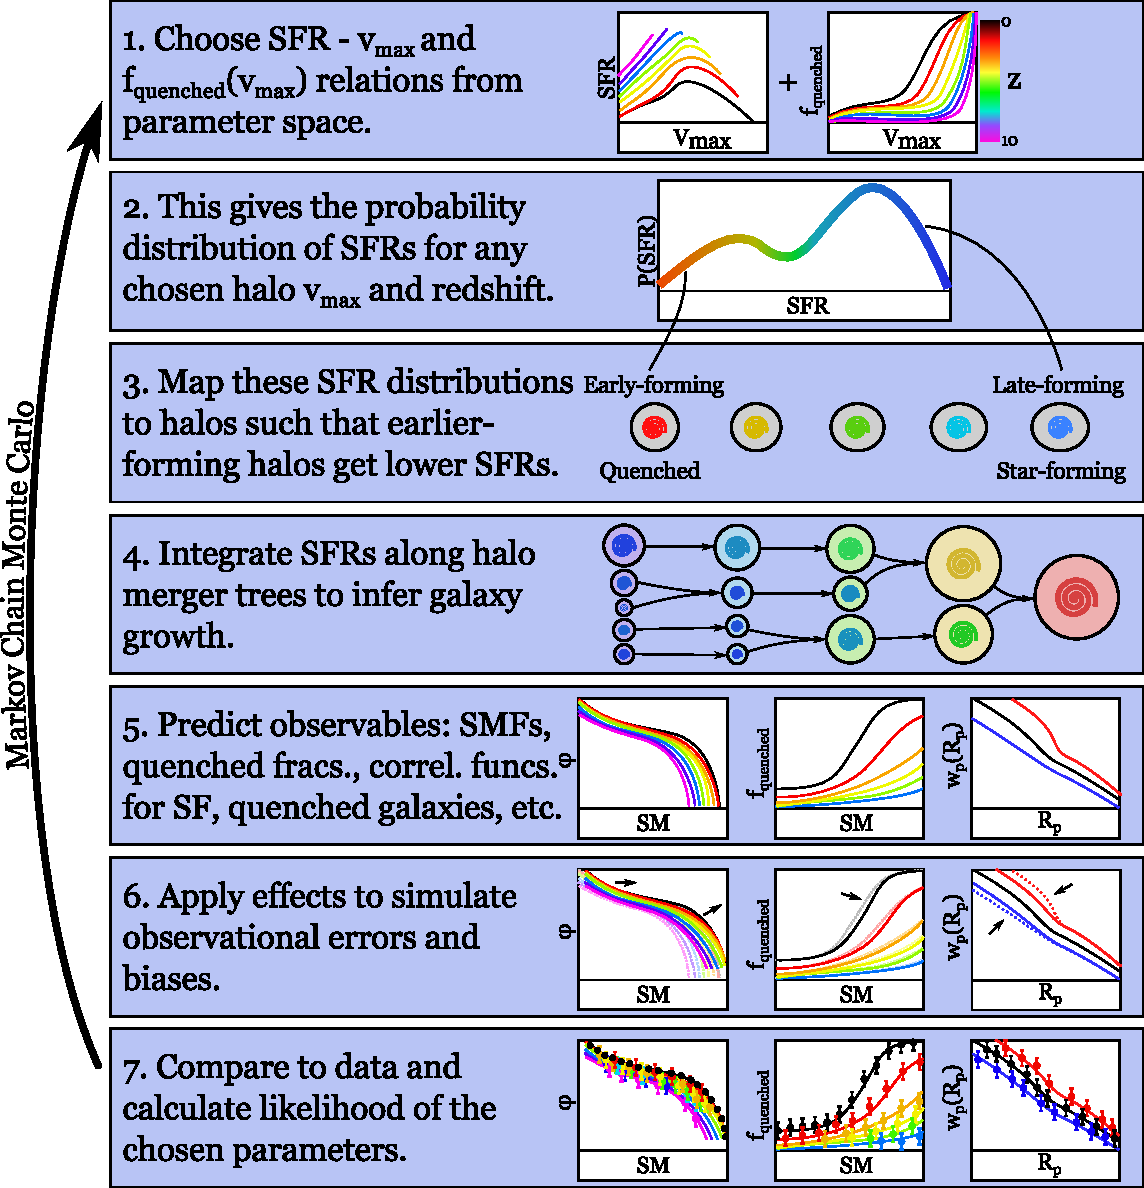
\includegraphics[width = \linewidth]{Figures/Chapter1/sfr_method.pdf}
    \caption{Image used with permission from: Peter Behroozi \cite{Behroozi2019UniverseMachine:010}}
    \label{fig:BehMeth}
\end{figure}


Using the iterative approach of parameter selection, mapping into halo structures, observable creation, through comparison to the observations the parameters are updated based on their likelihood and the process is iterated. This model is massively parallel allowing for over $10^{5}$ cores involved in any given parameter estimation. The model predictions are numerous included in which are in-situ vs ex-situ growth ratios in broad agreement with the other models.

\subsection{Limitations of the empirical technique}
%Drawbacks of SEM
Semi-empirical models as demonstrated above come in many different flavours. Each are able to draw conclusions about the connections that must exist between observational steps under given physical models. Whilst data is what empowers semi-empirical models it also presents one of semi-empirical models major limitations. Having wide and deep data sets which give statistically representative samples via large volumes to high redshift is difficult and costly. Most techniques involve correcting data sets and surveys to be consistent with one another creating a patchwork connecting the local and distant Universe. Semi-empirical models will continue to improve along with the available data although when built upon traditional dark matter simulations they share the volume constrains found in semi-analytic and hydro-dynamical models, however, this will continue to improve with increasing computational power.


\section{Galaxy Surveys Present and Future}
\label{sec:Surveys}
Galaxy surveys are the cornerstone of semi-empirical galaxy modelling, combined with dark matter simulations they form the basis of abundance matching. Other properties such as star formation, colour, shape, size, position, e.t.c. can all form either inputs to or constraints for the output for semi-empirical models. It therefore stands that improving the quality of models is predicated on improving the quality of the data.

\subsection{Past and Ongoing Surveys}
Present surveys as important to semi empirical models come in two forms 'wide' and 'deep'. Wide surveys look to cover a large area of the sky to get a statistically significant look at the galaxy population. Deep surveys cover a much smaller area but using longer exposure can observe much fainter objects. The trade-off between width and depth is visualised in by a simple example in Figure \ref{fig:WvD}. Tight surveys collect more photons per unit area and can therefore see to greater depth.

\begin{figure}[h]
    \centering
    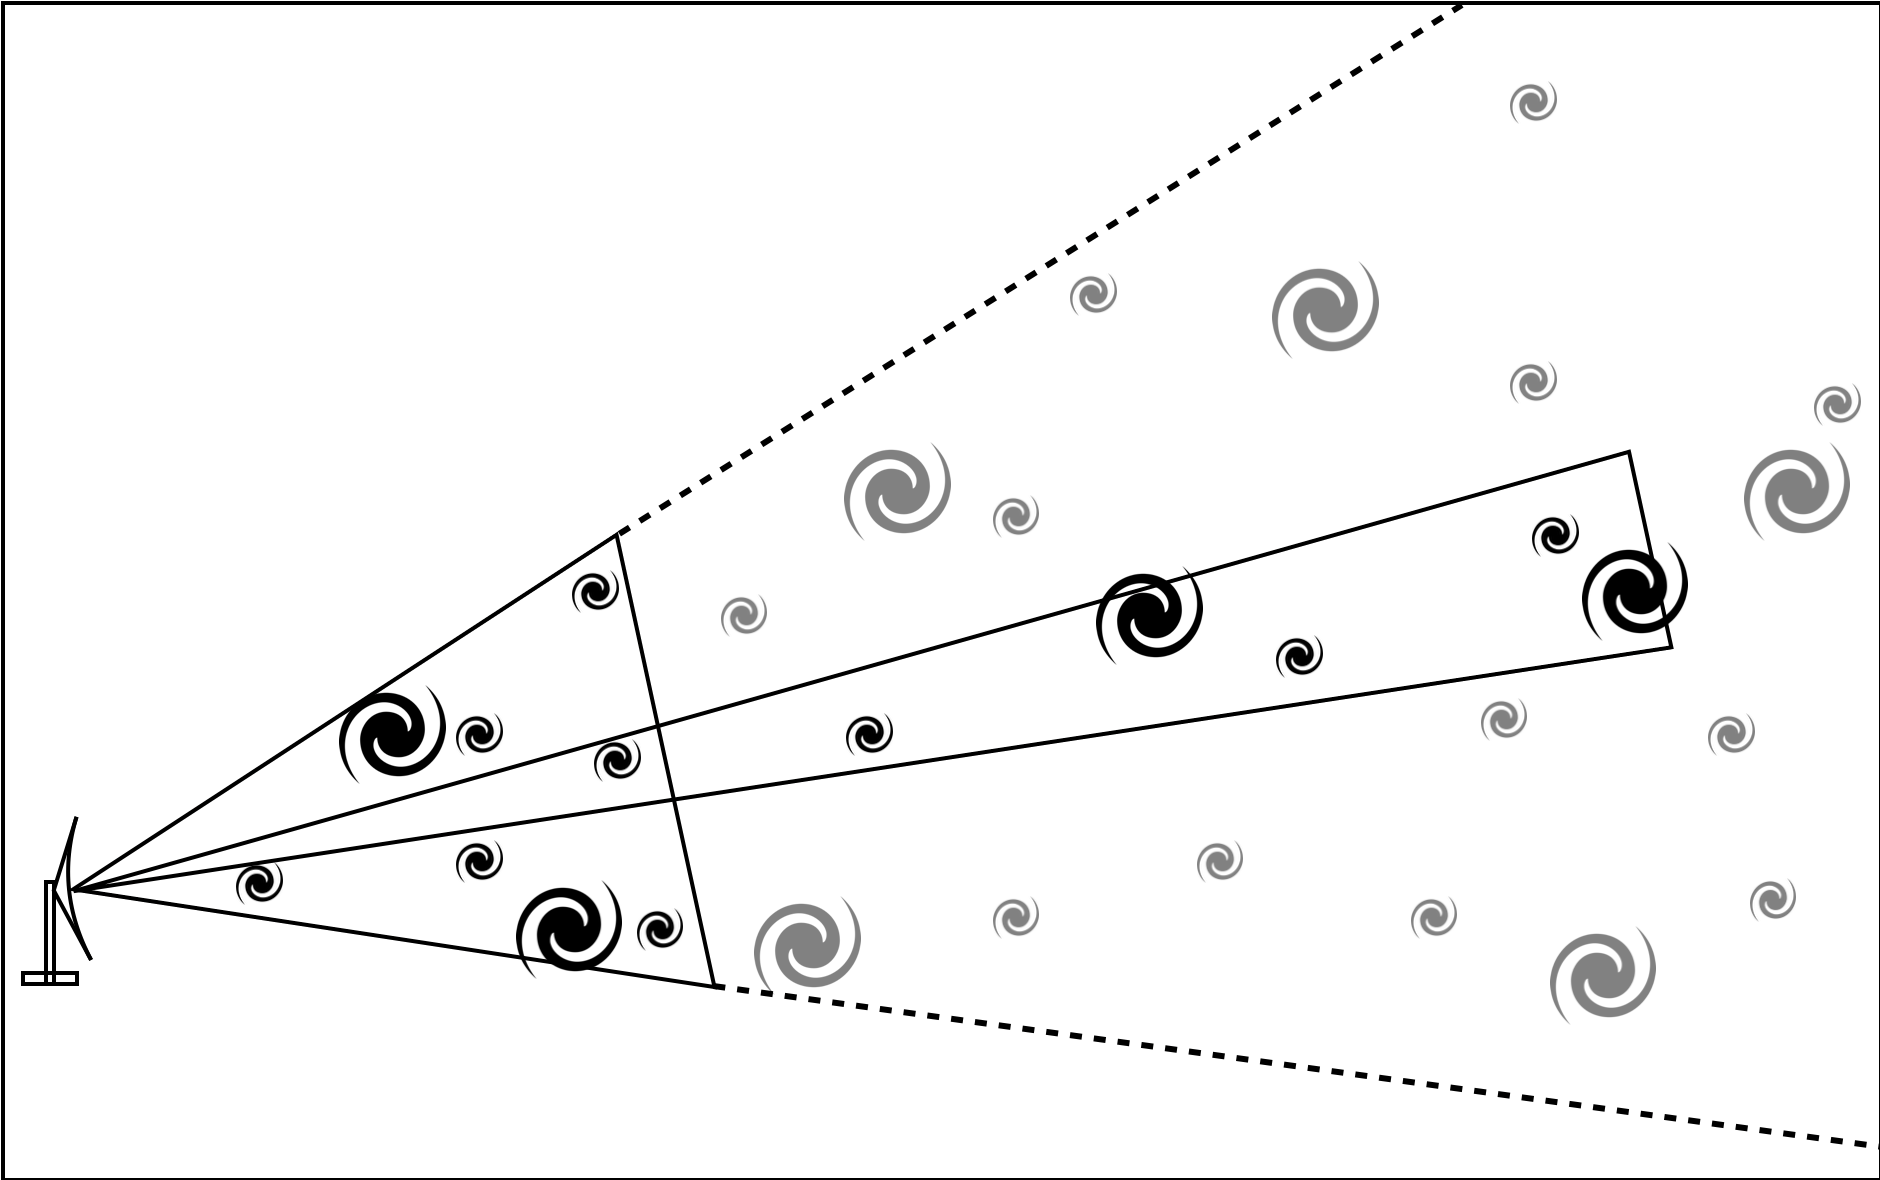
\includegraphics[width = \linewidth]{Figures/Chapter1/W_v_D_Toon.png}
    \caption{A simplified visualisation of how a trade off is made between width and depth in surveys. Given two observation areas the telescope is able to pick up galaxies to a much greater depth in narrow observation. By spending more time on one area of the sky the telescope can pick up more photons and therefore observe to a greater depth.}
    \label{fig:WvD}
\end{figure}

In addition larger galaxies are significantly brighter, the example in Figure \ref{fig:Vmax} uses two galaxy size examples. The smaller galaxies can be observed to the solid line and the larger galaxies to the dashed line. The telescope observes 6 small galaxies and 5 large galaxies, however as the larger galaxies are brighter and can be seen to greater depth. Corrections are therefore made to the number density of galaxies based on the depth that the galaxy can be observed to. In the 2D example from Figure \ref{fig:Vmax} the small galaxies can be seen in an area given by the solid area which we can call 1 unit$^2$ the larger galaxies can be seen in an area given by the dashed area that is 4 unit$^2$. In this example the smaller galaxies have a number density 6 galaxies p.u. area, the larger galaxies 1.25 galaxies p.u. area.

\begin{figure}[h]
    \centering
    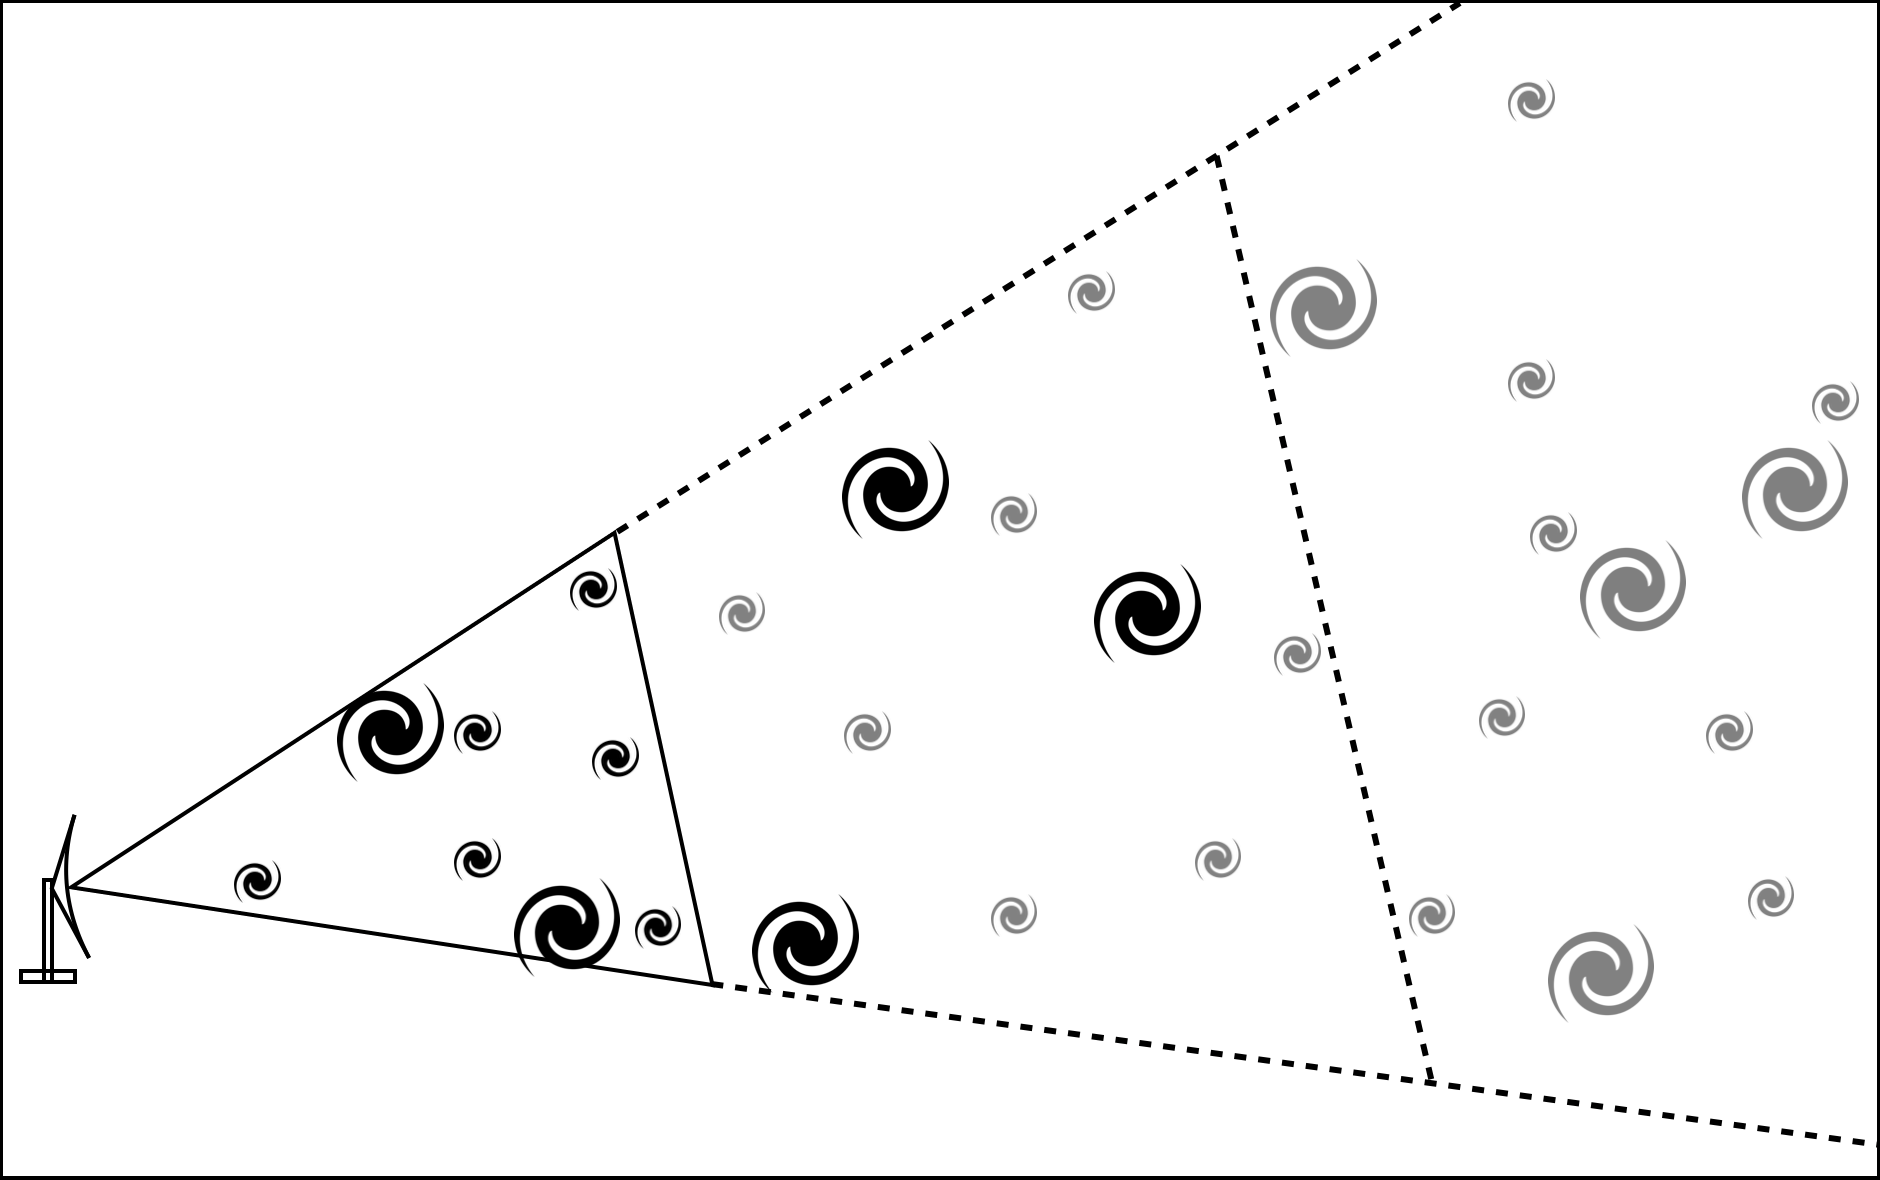
\includegraphics[width = \linewidth]{Figures/Chapter1/Vmax_Toon.png}
    \caption{A simplified visualisation of how the brightness of galaxies effects the observation depth. The smaller dimmer galaxies can be seen in the solid cone, larger and brighter galaxies can be seen up to the limits of the dashed cone.}
    \label{fig:Vmax}
\end{figure}

For each galaxy luminosity observed in a survey a correction must be made by the total depth it could have been observed to and the associated volume. In this way the volumetric density correction can be calculated for each galaxy in a given survey.

\subsubsection{Sloan Digital Sky Survey (SDSS)}

The Sloan Digital Sky Survey (SDSS) is arguably the premier wide survey for galaxies. SDSS started in 1998 with the mission to catalogue and map as much of the universe as possible. The latest release of the fourth phase is SDSS-DR19 \citep{AhumadaDamsted61} now includes one-third of the night sky, it covers (u,g,r,i,z) wavelengths, has over 1.2 billion objects including over 200 million galaxies.

\subsubsection{CANDLES}
CANDLES (The Cosmic Assembly Near-infrared Deep Extragalactic Leagacy Survey) observed galaxies in the redshift range z = 8 to 1.5. CANDLES uses three Hubble Space Telescope (HST) cameras to capture emission from mid-UV to near-IR for 250,000 galaxies. The primary goals of this survey of interest to this thesis is the observation of the peak of starformation and AGN activity at $z \simeq 2$ \cite{Grogin2011Candels:Survey}.

\subsubsection{COSMOS}

COSMOS: The Cosmic Evolution Survey is a 2 square degree survey covering many wavelengths using a combination of observation from many space based and ground based telescopes (Space: Hubble, Spitzer, GALEX, XMM, Chandra, Herschel, NuStar) (Ground: Keck, Subaru, VLA, ESO-VLT, UKIRT, NOAO, Badde and Blanco, CFHT). Combining the data allows cosmos to create a rich view of the observed objects across a huge range of wavelengths. COSMOS was designed to observe galaxy evolution across cosmic time and understand the environmental effects of galaxies growing in groups and clusters \citep{HomeCOSMOS}.

\subsubsection{3D-HST}

Using 248 orbits and 124 pointings the 3D-HST is a highly complementary survey observing 625 arcminuites of previously observed extra-galactic fields \citep{Brammer20123D-HST:Telescope}. 3D-HST provides spectroscopic redshifts for over 10,000 galaxies in the range $1 < z < 3.5$. The survey provides 22 bands of rest frame colours used for the redshift catalogs, the UV-IR star formation rates and, stellar masses. The primary science goal is to investigate the evolution of galaxies at high redshifts and in combination with CANDLES be the primary spectroscopic data set until the launch of JWST.

\subsection{Future Surveys}

Due to the pace of technological advancement and the difficult and expensive nature of building (and launching in the case of space based missions) telescopes our current survey telescopes are far behind what is theoretically possible. In this subsection to of the next generation survey telescopes are described, both are space based missions being launched into orbit at the second Lagrange\footnote{The Lagrange points are 5 distinct points in a gravitational two body system at which an object can remain at rest relative to the two major bodies. In these points the forces of gravitational acceleration, centripetal acceleration and for some points the Coriolis effect are all in balance.} point 4 times the distance of the moon away from earth. The second Lagrange point is unique in its position as it sits behind the earth and is therefore permanently in the earths shadow. This positioning is ideal for satellites as it is also within the earths magneto tail and therefore experiences lower solar wind irradiation. The drawback of this point is that from here any faults that are present at launch or develop during the operation of the missions will be permanent as it is not possible to retrieve and/or fix objects sent to these points.

\subsubsection{JWST \cite{JamesNASA}}

The James Webb Space Telescope is a cold infrared telescope with a planned launch in 2021\footnote{Correct at time of writing, JWST has some notoriety for pushing this date back}. Using multi-object near-infrared spectroscopy JWST will be able to take spectra for ~100 galaxies simultaneously. Galaxies will be observed in the redshift range $1 < z < 7$ covering the peak or cosmic starformation and much of their early formation. JWST as an infrared survey is suited to looking at the starformation of galaxies, buildup of the Hubble sequence, formation of metals, effects of starbursts are all among the observational capabilities of the telescope \cite{Windhorst2009JWST2009}.  


\subsubsection{EUCLID}

The EUCLID satellite will carry two instruments VIS \& NISP between them they will cover from 500nm to 2000nm wavelengths down to the 24th magnitude, providing images of galaxies up to redshift 2. Euclid will survey 15,000 deg$^2$ of the sky and then perform a deep survey covering 40 deg$^2$ to 2 magnitudes deeper. The primary mission goals of Euclid are to address open questions on dark matter, dark energy, cosmic expansion and the formation of large scale structures \cite{Amendola2018CosmologySatellite}. To address these questions galaxies will be used as tracers of dark matter that can provide tests of cosmological models, to do this the EUCLID pipeline will contain advance galaxy cluster detection algorithms \cite{EuclidCollaboration2019EuclidSelection}. 

\section{Original Sources}

A large fraction of this thesis is a restructuring of three papers published during PhD studies by PJG. The papers are:
\begin{itemize}
    \item \textit{`A Statistical Semi-Empirical Model: Satellite galaxies in Groups and Clusters'}  \citet{Grylls2019AClusters}, hereafter \Paper{1}
    \item \textit{`Predicting fully self-consistent satellite richness, galaxy growth and starformation rates from the STastical sEmi-Empirical modeL \textsc{steel}.'} \citet{Grylls2020PredictingSTEEL}, hereafter \Paper{2}
    \item \textit{`The significant effects of stellar mass estimation on galaxy pair fractions.'} \citet{Grylls2020TheFractions}, hereafter \Paper{3}
\end{itemize}

Each chapter, including the introduction and conclusion may contain work from all three sources however the major sources for each are as follows: Chapter \ref{Chapter:Method} reports primarily from \Paper{1} where the method was originally published, updates to the method from \Paper{2} \& \Paper{3} are also included. Chapter \ref{Chapter:GalDist} restructures the discussion of galaxy distributions from \Paper{1} \& \Paper{2}. Chapter \ref{Chapter:GalGrowth} presents the critical finding published in \Paper{2} and contextualises the main result in greater detail. Finally Chapter \ref{Chapter:GalPairs} details the results from \Paper{3} and a work in preparation by SP for which PJG has acted as a supervisor in conjunction with FS. Where possible text and figures are reproduced in original form, however substantial reordering, alongside edits and additions have been selectively made to show how the work produced over PJG's candidature relate to one another and the wider field.  
